\documentclass[11pt,twoside]{article}

% =============================================================
% PACKAGES
% =============================================================
\usepackage[utf8]{inputenc}
\usepackage[T1]{fontenc}
\usepackage{lmodern}
\usepackage{microtype}
\usepackage[english]{babel}

\usepackage[a4paper,
            left=2.0cm, right=2.0cm,
            top=2.4cm, bottom=2.4cm,
            headheight=14pt]{geometry}

\usepackage{fancyhdr}
\pagestyle{fancy}
\fancyhf{}
\fancyhead[LE,RO]{\small\itshape Heterogeneous supervision and evaluation validity in cancer assertion extraction}
\fancyfoot[C]{\small\thepage}
\renewcommand{\headrulewidth}{0.4pt}

\fancypagestyle{plain}{%
  \fancyhf{}
  \fancyfoot[C]{\small\thepage}
  \renewcommand{\headrulewidth}{0pt}
}

\usepackage{amsmath,amssymb}
\usepackage{booktabs,tabularx,multirow,array,makecell}
\renewcommand{\arraystretch}{1.15}
\usepackage{graphicx,caption,subcaption,float}

\renewcommand{\topfraction}{0.85}
\renewcommand{\bottomfraction}{0.70}
\renewcommand{\textfraction}{0.15}
\renewcommand{\floatpagefraction}{0.65}

\captionsetup{font=small,labelfont=bf,labelsep=period,skip=6pt}
\captionsetup[table]{position=top}
\captionsetup[figure]{position=bottom}

\usepackage{xcolor}
\definecolor{linkblue}{RGB}{0,70,160}
\definecolor{citeblue}{RGB}{0,100,180}
\usepackage[colorlinks=true,
            linkcolor=linkblue,
            citecolor=citeblue,
            urlcolor=linkblue,
            breaklinks=true,
            bookmarks=true,
            bookmarksnumbered=true,
            pdftitle={Heterogeneous supervision and evaluation validity in cancer assertion extraction}]{hyperref}
\usepackage{xurl}

\usepackage{titlesec}
\usepackage{enumitem}
\setlist[itemize]{leftmargin=1.5em,itemsep=2pt,parsep=0pt,topsep=4pt}
\setlist[enumerate]{leftmargin=1.5em,itemsep=2pt,parsep=0pt,topsep=4pt}

\usepackage[hang,flushmargin]{footmisc}
\setlength{\footnotemargin}{0.8em}

\setlength{\parskip}{0.4em}
\setlength{\parindent}{1.2em}
\setlength{\emergencystretch}{2.5em}

\setlength{\textfloatsep}{12pt plus 3pt minus 3pt}
\setlength{\floatsep}{10pt plus 2pt minus 2pt}
\setlength{\intextsep}{10pt plus 2pt minus 2pt}

\usepackage[numbers,sort&compress]{natbib}

% =============================================================
% CUSTOM COMMANDS
% =============================================================
\newcommand{\shead}[1]{\textsc{#1}}
\newcommand{\code}[1]{\texttt{#1}}
\newcommand{\model}[1]{\texttt{#1}}

% =============================================================
% TITLE BLOCK
% =============================================================
\title{%
  \textbf{Heterogeneous supervision and evaluation validity \\
          in cancer assertion extraction}
}

\author{%
  Freddie Yu\,$^{1}$,
  Michael Tillich\,$^{3}$,
  Martin Baron\,$^{3}$,
  Zahraa Abdallah\,$^{2}$,
  Yi Liu\,$^{1,*}$,
  Tom Gaunt\,$^{1}$
  \\[6pt]
  \begin{minipage}{0.92\textwidth}\centering\small
    $^{1}$MRC Integrative Epidemiology Unit, Bristol Medical School,
    University of Bristol, Bristol, BS1 5DS, UK \\
    $^{2}$School of Engineering Mathematics and Technology,
    University of Bristol, Bristol, UK \\
    $^{3}$F.\ Hoffmann-La Roche Ltd, Grenzacherstrasse 124,
    4070 Basel, Switzerland
  \end{minipage}
}

\date{}

% =============================================================
% DOCUMENT
% =============================================================
\begin{document}

\maketitle
\thispagestyle{plain}

\begin{abstract}
% =============================================================
% STRUCTURED ABSTRACT for JAMIA Research and Applications
% (≤250 words; five headings:
%  Objective / Materials and Methods / Results / Discussion /
%  Conclusion).
% This file expands inside \begin{abstract}...\end{abstract}.
% =============================================================

\noindent\textbf{Objective.}
In cancer knowledge-base (KB) curation, models are typically
selected by public benchmark scores. We test whether benchmark F1
predicts KB-surfacing yield in a pre-registered factorial study.

\noindent\textbf{Materials and Methods.}
We trained 310 models across two waves: a schema-comparison wave
(4 encoders \(\times\) 3 schemas \(\times\) 10 seeds = 120 runs)
selecting the operational relation schema, and a configuration
wave (3 encoders \(\times\) 3 training schedules \(\times\) 20
seeds + a 10-seed RoBERTa-base reference = 190 runs) under that
schema. Each model was evaluated against 162 curator-validated
CIViC oncology assertions. Analyses comprised
pre-registered paired-difference contrasts on three KB-audit
metrics, a variance decomposition by design lever, and the
rank-inversion rate among benchmark-tied configuration pairs.

\noindent\textbf{Results.}
An entity-pair schema improved KB surfacing over a coarser family
schema (\(\Delta=+0.117\), 95\% paired-bootstrap CI [+0.045, +0.194]).
Multi-corpus training improved out-of-domain generalisation on
BC5CDR drug--disease F1 (\(\Delta=+0.139\), Cohen's \(d=2.04\)).
Encoder, schedule, and their interaction explained about five
times more variance in KB argmax accuracy than in BioRED ex-NEG F1
(\(R_B=0.21\); cluster-bootstrap 95\% CI [0.028, 0.990]), with the
training-schedule term contributing most of the gap.
Among 18 benchmark-tied configuration pairs the rank-inversion rate
was 0.50 (95\% CI [0.14, 0.83]).

\noindent\textbf{Discussion.}
Benchmark F1 and KB yield diverged most in the training-schedule
arm: half of benchmark-tied configuration pairs reversed their KB
ranking. Wide confidence intervals at the realised cell counts
limit directional claims for the coupling-slope family.

\noindent\textbf{Conclusion.}
Benchmark scores alone are insufficient for oncology KB curation
pipelines. We recommend pairing benchmark scoring with a
lightweight KB-anchor audit on 100--200 curator-validated
assertions; the audit code and pre-registration are released.

\end{abstract}

\smallskip
\noindent\textbf{Keywords:}
natural language processing;
knowledge bases;
medical oncology;
reproducibility of results;
research design

\vspace{1.0em}

% =============================================================
% MAIN TEXT
% =============================================================
\section{Background and Significance}
\label{sec:background}

% Para 1: clinical motivation
Cancer knowledge bases such as the Clinical Interpretation of
Variants in Cancer (CIViC) \citep{griffith2017civic} depend on
expert curation to keep pace with growing oncology literature.
Like OncoKB \citep{chakravarty2017oncokb} and CancerMine
\citep{lever2019cancermine}, CIViC records curator-validated
drug, gene, variant, and disease assertions with their supporting
evidence; manual curation, however, lags the rate at which new
publications are indexed in PubMed \citep{civicfact2025}. Pretrained
biomedical encoders, most prominently PubMedBERT
\citep{gu2021pubmedbert} and BioLinkBERT
\citep{yasunaga2022biolinkbert}, are increasingly used to flag
candidate assertions for curator review at scale.

% Para 2: the unexamined assumption + evaluation literature gap
Models are typically selected by their performance on public
relation-extraction benchmarks: macro-averaged F1 score (macro-F1)
on BioRED \citep{luo2022biored}, BC5CDR drug--disease F1
\citep{li2016bc5cdr}, and component scores in suites such as the
Biomedical Language Understanding and Reasoning Benchmark
(BLURB) \citep{gu2021pubmedbert}. The implicit assumption is that
benchmark performance predicts downstream KB yield. To our
knowledge, this assumption has not been tested on a
curator-validated oncology knowledge base. Construct-validity
audits \citep{bowman2021construct} and evidence-centred benchmark
designs \citep{liu2024ecbd} have shown that benchmark improvements
need not imply meaningful capability gains, but those critiques
address general-domain language understanding rather than
biomedical curation.

% Para 3: biomedical NLP gap
Within biomedical NLP, benchmark suites (BLURB
\citep{gu2021pubmedbert}; BigBIO \citep{fries2022bigbio}) and
KB-curation pipelines (CIViCmine \citep{lever2019civicmine} for
variant mining; BioREx \citep{lai2023biorex} for multi-corpus
relation extraction) have developed in parallel. No study in
either body of work has tested whether benchmark-selected pipelines
optimise downstream KB yield in oncology.

% Para 4: LLM-era context and encoder-only scoping
Decoder-only large language models are now competitive with
fine-tuned encoders on biomedical relation tasks
\citep{chen2025nlpbench} and have been evaluated on BioRED and
CIViC-Fact \citep{civicfact2025}. We restricted the study to
encoder-only models because their inference pipeline and output
distribution are homogeneous across the four encoder families
compared here, so a variance decomposition can isolate encoder,
schedule, and schema effects without confounding from prompt
design or decoding configuration. The architectural diversity of
current LLMs is a separate design axis that the present factorial
cannot identify; we mark its extension as a stated follow-up
(\S\ref{sec:discussion}).

% Para 5: contributions and RQs
To close this gap, we ran a pre-registered factorial study of 310
training runs across four encoders, three nested relation schemas,
and three training schedules, evaluated against 162
curator-validated CIViC assertions. Benchmark and KB performance
are treated as two evaluation axes to be compared rather than
merged onto a single ranking
\citep{lawlor2017triangulation,liugaunt2024asq}, and the
contribution of each design lever is partitioned across the two
axes by a variance decomposition. Four research questions follow:
whether a finer relation schema improves KB surfacing (RQ1);
whether encoder scale, multi-corpus training, or
oncology-projected staging improves generalisation (RQ2); whether
encoder rankings are stable across three KB-audit metrics (RQ3);
and whether benchmark and KB rankings diverge under matched
configurations (RQ4).

\section{Materials and Methods}
\label{sec:methods}

% =====================================================
\subsection{Data sources}
\label{sec:data}

The task is relation extraction at the abstract level: given a PubMed
abstract and two pre-identified entity spans, predict the relation
type from a schema vocabulary (or \code{\_\_NEGATIVE\_\_} if no
relation holds). We trained on three public corpora: BioRED
\citep{luo2022biored} (600 abstracts, multiple relation types across
gene, disease, variant, and chemical entities; 500/100
train-dev/test split); DrugProt \citep{miranda2023drugprot}
(4{,}250 documents, thirteen chemical--protein mechanism relations);
and BC5CDR \citep{li2016bc5cdr} (1{,}000 train+dev + 500 test
documents, binary chemical-induces-disease relations).

The knowledge-base anchor was CIViC \citep{griffith2017civic}. We
extracted 165 evidence-supported targets (PubMed abstract plus two
entity spans). Of these, 162 mapped to schema vocabularies under
the family-to-label projection described in \S\ref{sec:kb-audit}
and form the evaluable target pool; the remaining three carry
variant--gene endpoints not covered by any of the three schema
vocabularies and are documented as a structural coverage gap. An
oncology-projected training subset comprised 733 abstracts whose
PubMed records carry a Medical Subject Headings (MeSH) C04
(Neoplasms) descriptor \citep{lipscomb2000mesh}. Corpus details are
in Supplement~B.

% =====================================================
\subsection{Schema design}
\label{sec:schema}

Three nested relation schemas were defined at increasing granularity.
The 4-label \shead{family} schema (S\textsubscript{family}) is the
minimum partition preserving three clinical pair-type categories:
drug--disease, drug--gene regulation, and other associations.%
\footnote{S\textsubscript{family} is named \texttt{S\_flat} in the
pre-registration document and analysis code; we rename it here for
readability.} The
8-label \shead{pair} schema (S\textsubscript{pair}) decomposes the general-association category into
entity-pair-specific categories (\code{GENE\_DISEASE},
\code{VARIANT\_DISEASE}, etc.), recovering the entity-pair
distinctions that BioRED natively annotates. The 13-label
\shead{mechanism} schema (S\textsubscript{mech}) further decomposes
drug--gene regulation into five DrugProt sub-mechanisms. A relation is eligible for training and evaluation only if its
entity-pair type is covered by the schema. Schema vocabularies,
legal-pair filters, and the projection used in the KB audit are in
Supplement~C.

% =====================================================
\subsection{Training protocol}
\label{sec:training}

Four encoders were trained: PubMedBERT-base
\citep{gu2021pubmedbert}, BioLinkBERT-base
\citep{yasunaga2022biolinkbert}, PubMedBERT-large
\citep{gu2021pubmedbert}, and a general-domain reference
(RoBERTa-base \citep{liu2019roberta}). Three training schedules were
compared: single-corpus (BioRED only); multi-corpus joint (BioRED +
DrugProt + BC5CDR in one stage); and oncology-projected staged, in
which a continuation stage on the MeSH-C04 subset followed the
multi-corpus stage. Each training stage used a fixed budget of
2{,}048 optimiser updates with a cap of 2{,}000 positive rows per
corpus shard. The staged schedule consumed 4{,}096 updates in
total, so pairwise contrasts within an encoder compare schedule
composition rather than total compute. All runs share the same
optimiser, learning rate, and early-stopping criterion (full
hyperparameter inventory in Supplement~D).

The study comprised two waves. The \emph{schema-comparison wave}
($n = 120$ runs) varied schema and encoder under a fixed schedule
to select the operational schema (RQ1). The \emph{configuration
wave} ($n = 180$ main runs plus a 10-seed RoBERTa-base reference
cell, 190 total) fixed schema to the first-wave selection and
varied encoder $\times$ schedule with 20 seeds per cell,
addressing RQ2, RQ3, and RQ4. Seed indices 1--10 are shared across
the two waves so that cross-wave paired contrasts can match;
indices 11--20 are used in the configuration wave only.
Hyperparameters and seeding policy are in Supplement~D.

A pre-registered parameter-efficient fine-tuning arm based on
low-rank adaptation \citep[LoRA;][]{hu2022lora} (rank 16; attention
query and value projections; classifier head fully trained)
collapsed to uniform negative prediction under all three
pre-committed configurations and was declared a methodological null
(Supplement~I).

% =====================================================
\subsection{Knowledge-base audit}
\label{sec:kb-audit}

Each of the 162 CIViC targets carries a PubMed abstract, two
pre-identified entity spans, and a curator-recorded relation that
maps to one or more schema-vocabulary labels under a heuristic
family-to-label projection. Because entity spans are pre-identified,
the audit isolates relation-type discrimination rather than entity
recognition. The projection maps each (entity-pair family, CIViC
evidence-type, schema) tuple to an expected-label set, which is
set-valued when the CIViC evidence type is compatible with more
than one schema label; the full projection rules and the released
JSON are in Supplement~C.

\paragraph{Inter-annotator audit.}
We audited the heuristic projection against an independent second
annotator on a stratified random sample of 30 of the 162 evaluable
targets (18.5\%). The second annotator was a large language model
(Claude Opus 4.7, \texttt{temperature\,=\,0}, deterministic
decoding) prompted with the same label definitions but blind to the
heuristic's output \citep{gilardi2023llmannotator}. The resulting
$\kappa$ is a model-based validity check rather than a
human--human inter-annotator estimate, and is reported as a lower
bound on agreement with an expert human curator. Observed agreement
was \(\kappa = 0.56\) (95\% CI [0.32, 0.80]); all seven
disagreements followed a single directional pattern detailed in
\S\ref{sec:results-iaa}. Per-target rationales are in Supplement~C.

\paragraph{KB-audit metrics.}
For each model on each target we computed three correctness-aware
metrics: (i)~\textbf{KB argmax accuracy} (primary): 1 if the
model's top-ranked label is in the expected-label set, 0 otherwise;
(ii)~\textbf{KB truth probability}: the model's predicted
probability summed over labels in the expected set; and
(iii)~\textbf{KB selective-recall AUC}: the area under the curve of
per-target precision against rejection fraction, computed by
sweeping a confidence threshold and abstaining on predictions below
it. Intuitively, (i) asks whether the model's top prediction is
right, (ii) asks how much probability mass landed on truth, and
(iii) asks how reliably the model abstains when wrong. KB argmax
accuracy was the pre-registered primary metric; KB truth probability
and KB selective-recall AUC are reported as discrimination and
selective-prediction sensitivity analyses (\S\ref{sec:results-rq3}).
Formal definitions are in Supplement~C.

\paragraph{External benchmarks.}
The primary external benchmark is the macro-averaged F1 score
(macro-F1) of BioRED over its non-negative labels (BioRED ex-NEG);
BC5CDR drug--disease F1 is the out-of-domain benchmark.

% =====================================================
\subsection{Statistical analysis}
\label{sec:stats}

\paragraph{Target estimands.}
Each contrast estimates the observed effect of one design lever
across the realised factorial cells, with seeds treated as
nuisance variation; we do not extrapolate variance shares to a
wider population of encoders or schedules.

\paragraph{Reliability of the primary KB metric.}
KB argmax accuracy is noisier across seeds than the external
benchmarks. On the configuration wave (9 cells $\times$ 20 seeds),
the intraclass correlation (one-way random effects; ICC(1,1)
\citep{shrout1979intraclass}) for KB argmax accuracy was 0.67,
indicating substantial between-cell separation, but the pooled
within-cell standard deviation was 0.17 --- about three times the
within-cell standard deviation for BioRED ex-NEG F1 over the same
nine cells (0.06). Pre-registered seed-paired contrasts
absorb cell-level noise into the within-cell difference and were
specified for every KB-side comparison; the residual seed-level
dispersion still widens paired-bootstrap intervals at the realised
cell counts and is the precision constraint behind reporting the
coupling-slope family descriptively (\S\ref{sec:results-rq4}).

\paragraph{Comparison protocol.}
The locked primary family contained 21 planned comparisons
(Supplement~K). After H4 (LoRA) was declared a methodological null
and H5 (architecture) was deferred, the realised analysis covers 15
comparisons: nine paired-difference contrasts entered into the
Benjamini--Hochberg family (H1$\,$two encoder-scale contrasts;
H2$\,$one multi-corpus contrast; H3$\,$six staging contrasts), five
coupling slopes (H6, reported descriptively), and one variance
ratio (H7). The paired-difference contrasts use
Benjamini--Hochberg false-discovery-rate adjustment
\citep{benjamini1995controlling} at \(q=0.05\); each reports both
paired \(t\) and Wilcoxon signed-rank
\citep{wilcoxon1945individual}, with paired \(t\) as headline.
Paired-bootstrap 95\% confidence intervals (\(B=10{,}000\)) resample
within-cell differences across seeds and form the primary
uncertainty estimate.

\paragraph{Variance decomposition.}
For each wave we partitioned the sum-of-squares of BioRED ex-NEG F1
and of KB argmax accuracy across design factors using a Type-I
analysis of variance (sequential fits in the pre-registered factor
order; Supplement~K). The variance ratio \(R\) is the ratio of the
design-lever variance share in the benchmark metric to the same
share in the KB metric: \(R<1\) means the same design levers
explain more KB variance than benchmark variance, and \(R>1\)
inverts that direction. \(R_B\) is accompanied by a
cluster-bootstrap 95\% CI (5{,}000 cell-level resamples). We also
report the rank-inversion rate: the fraction of configuration-wave
cell pairs whose BioRED ex-NEG F1 differs by less than the
pre-registered matching radius \(\rho=0.03\) (one schema-wave
within-cell BioRED SD) and whose KB rankings disagree. A sensitivity
sweep over \(\rho\in\{0.01, 0.03, 0.05\}\) is in Supplement~H.

% =====================================================
\subsection{Pre-registration and protocol deviations}
\label{sec:prereg}

The factorial design, hypotheses, decision rules, and
multiple-comparison tiering were pre-registered
\citep{nosek2018preregistration} before any configuration-wave run.
The pre-registration document and amendment log are in the Data and
Code Availability statement.

Three post-lock amendments were documented in the versioned amendment
log. \emph{Amendment~1} (pre-unblinding): a slope-CI reportability
gate (\(\leq 0.30\) width) was added after the schema-comparison
wave revealed wider within-cell dispersion than assumed; the
variance-ratio factor set was also clarified.
\emph{Amendment~2}: the LoRA hypothesis (H4) was declared null
after all configurations collapsed; the architecture hypothesis
(H5) was deferred. During manuscript preparation we also
reclassified the PubMedBERT-base vs BioLinkBERT-base contrast,
originally listed under H1 encoder-scale, as an
architecture comparison rather than a scale comparison (both
encoders are base-scale; they differ in pretraining corpus and
initialisation). It is reported in Supplement~F alongside the
remaining H1 results but is not part of the encoder-scale family
in Table~\ref{tab:t2}, consistent with H5's deferred status.
\emph{Amendment~3}: the inter-annotator audit, the ICC analysis,
and the \(\rho\) sensitivity analysis were added as post-hoc
validity checks during manuscript preparation. No pre-registered
decision rule, threshold, or comparison tier was amended after
unblinding.

% =====================================================
\subsection{Computational environment}

Training and evaluation ran on the University of Bristol's BriCS
Isambard-AI system under Slurm; the pinned software environment is
in Supplement~A.

\section{Results}
\label{sec:results}

% =====================================================
\subsection{Schema selection (RQ1)}
\label{sec:results-rq1}

Pooled across encoders and seeds, the 8-label entity-pair schema
(S\textsubscript{pair}) was selected for the configuration wave.
KB argmax accuracy improved by \(\Delta=+0.117\) (paired 95\% CI
[+0.045, +0.194]; Cohen's \(d=+0.55\); permutation \(p=0.015\);
FDR-\(q=0.024\)) over S\textsubscript{family} and by
\(\Delta=+0.242\) (95\% CI [+0.171, +0.313]; \(d=+1.29\);
\(p<0.0001\)) over S\textsubscript{mech} (Table~\ref{tab:t1}).
S\textsubscript{pair} outperformed S\textsubscript{family} in every
encoder (\(\Delta\in\{+0.052, +0.127, +0.132, +0.159\}\)). The
13-label schema collapsed because five of its six
drug--gene-regulation categories had no positive examples in the
BioRED test set. Per-encoder bar charts are in Figure~\ref{fig:f1};
full per-schema results are in Supplement~E.

\begin{table}[!ht]
\centering
\caption{Schema-comparison wave: pairwise contrasts on
KB argmax accuracy, paired bootstrap (\(B=10{,}000\)) on
\(4\times10=40\) matched (encoder, seed) cells.}
\label{tab:t1}
\small
\begin{tabular}{@{}lcccc@{}}
\toprule
\textbf{Contrast} & \textbf{\(\Delta\)} & \textbf{95\% CI}
& \textbf{Cohen's \(d\)} & \textbf{Perm.\ \(p\)} \\
\midrule
S\textsubscript{pair} vs S\textsubscript{family}
  & $+0.117$ & $[+0.045, +0.194]$ & $+0.55$ & $0.015$ \\
S\textsubscript{pair} vs S\textsubscript{mech}
  & $+0.242$ & $[+0.171, +0.313]$ & $+1.29$ & $<0.0001$ \\
\bottomrule
\end{tabular}
\end{table}

\begin{figure}[!ht]
\centering
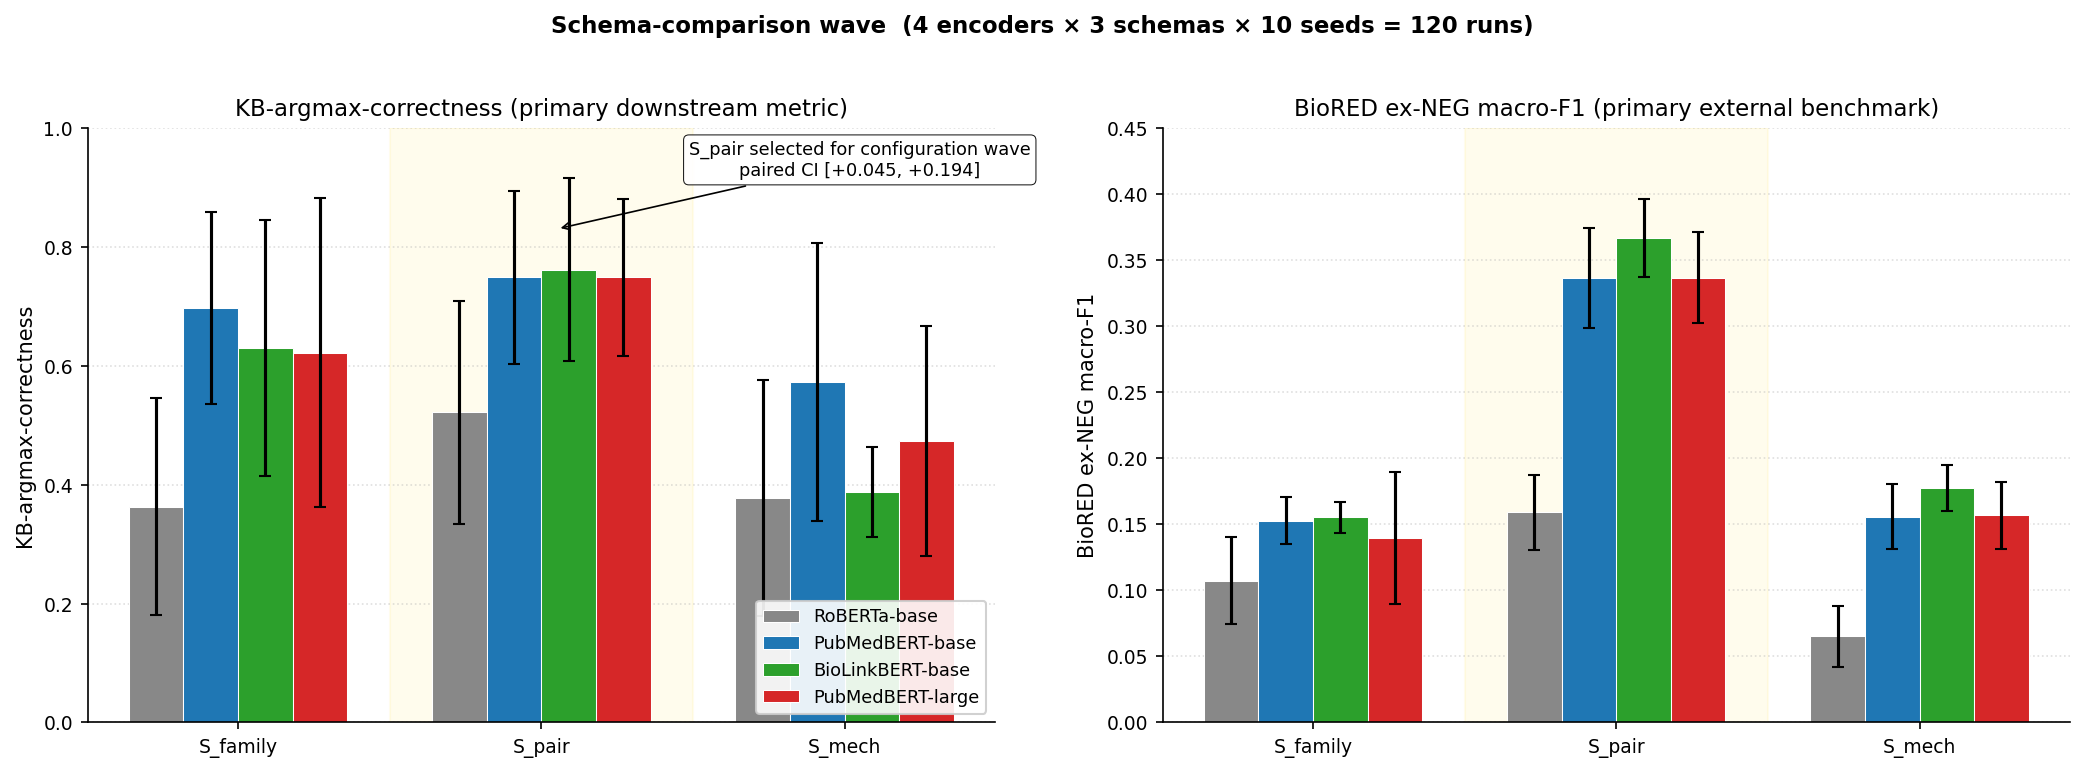
\includegraphics[width=\textwidth]{figures/fig1_schema_selection.png}
\caption{Schema-comparison wave: KB argmax accuracy (left) and
BioRED ex-NEG F1 (right) by encoder $\times$ schema. Bars are seed
means; error bars are within-cell SDs.}
\label{fig:f1}
\end{figure}

% =====================================================
\subsection{Inter-annotator audit}
\label{sec:results-iaa}

Inter-annotator agreement on a stratified 30/162 subset was
\(\kappa=0.56\) (95\% CI [0.32, 0.80]). All seven disagreements
followed a single directional pattern: the LLM annotator chose
\code{\_\_NEGATIVE\_\_} while the heuristic chose a positive
relation. The disagreements concentrated on EGFR-pathway
tyrosine-kinase inhibitors (gefitinib, erlotinib, lapatinib,
dacomitinib) and the HSP90 inhibitor tanespimycin; in six of seven
cases the CIViC-cited drug was not literally named in the abstract,
and in the seventh (gefitinib--EGFR, PMID 22370314) the gene side
was not named. The heuristic is therefore recall-favouring: it
labels too many of these abstracts as positive when one side of
the cited (drug, gene) pair is missing from the text. We retained
the heuristic unchanged and treat the audit as a directional
validity check (per-disagreement table in Supplement~C).

% =====================================================
\subsection{Training configurations (RQ2)}
\label{sec:results-rq2}

Of the nine pre-registered paired contrasts under
S\textsubscript{pair}, four confirmed, four were null, and one
marginal at \(q\approx0.05\) (Table~\ref{tab:t2}). At the family
level, the encoder-scale hypothesis (H1) was null, the
multi-corpus hypothesis (H2) was confirmed, and the staged-schedule
hypothesis (H3) was partial: 3 of 6 contrasts confirmed at
\(q<0.05\), which is the locked-design boundary between
``partial'' (2--3 of 6) and ``confirmed'' (\(\ge 4\) of 6).

\paragraph{Multi-corpus training.}
Multi-corpus joint training improved BC5CDR drug--disease F1 by
\(\Delta=+0.139\) (95\% CI [+0.108, +0.166]; Cohen's \(d=2.04\);
\(q<0.001\)) over single-corpus BioRED training at PubMedBERT-base.
The same direction held at BioLinkBERT-base (\(\Delta=+0.158\)) and
PubMedBERT-large (\(\Delta=+0.199\)).

\paragraph{Oncology-projected staging.}
Of six tests (three encoders \(\times\) two benchmarks), three
confirmed, one was marginal, and two were null. PubMedBERT-base
benefited on both benchmarks (BioRED ex-NEG \(\Delta=+0.053\),
\(q<0.001\); BC5CDR \(\Delta=+0.030\), \(q=0.007\)) and
BioLinkBERT-base on BioRED ex-NEG (\(\Delta=+0.023\), \(q=0.016\)).
PubMedBERT-large was marginal on BC5CDR drug--disease
(\(\Delta=+0.028\), \(q=0.047\)) and null on BioRED ex-NEG; staging
hurt no encoder on either benchmark. The staging benefit is real
but encoder- and benchmark-dependent.

\paragraph{Encoder scale.}
PubMedBERT-large did not outperform PubMedBERT-base
(\(\Delta=-0.008\), \(q=0.519\)) or BioLinkBERT-base
(\(\Delta=-0.021\), \(q=0.159\)) on BioRED ex-NEG. Across the
three training levers we tested, multi-corpus training produced the
largest and most reliable benchmark effect, staged continuation was
encoder-dependent, and encoder scale alone showed no benchmark
improvement at the realised cell counts. Per-cell results are in
Figure~\ref{fig:f2}; the nine paired contrasts and their CIs are in
Figure~\ref{fig:f3}; per-contrast statistics are in Supplement~F.

\begin{table}[!ht]
\centering
\caption{Configuration-wave primary-family hypothesis tests under
S\textsubscript{pair}. The Anchor column gives the
largest-magnitude paired contrast in each family. Cohen's $d$ is
$d_z$ on the paired-difference scale. Full per-contrast results
are in Supplement~F.}
\label{tab:t2}
\small
\begin{tabular}{@{}lcccp{3.5cm}@{}}
\toprule
\textbf{Test family} & \textbf{Conf.}
& \textbf{Null} & \textbf{Marg.} & \textbf{Anchor \(\Delta\) (\(d_z\))} \\
\midrule
Encoder-scale (H1; 2)    & 0 & 2 & 0 & --- \\
Multi-corpus (H2; 1)     & 1 & 0 & 0 & $+0.139$, $d_z\!=\!2.04$ (BC5CDR DD) \\
Staged schedule (H3; 6)  & 3 & 2 & 1 & $+0.053$, $d_z\!=\!0.87$ (BioRED ex-NEG) \\
\midrule
\textbf{Total (9)}       & \textbf{4} & \textbf{4} & \textbf{1} & \\
\bottomrule
\end{tabular}
\end{table}

\begin{figure}[!ht]
\centering
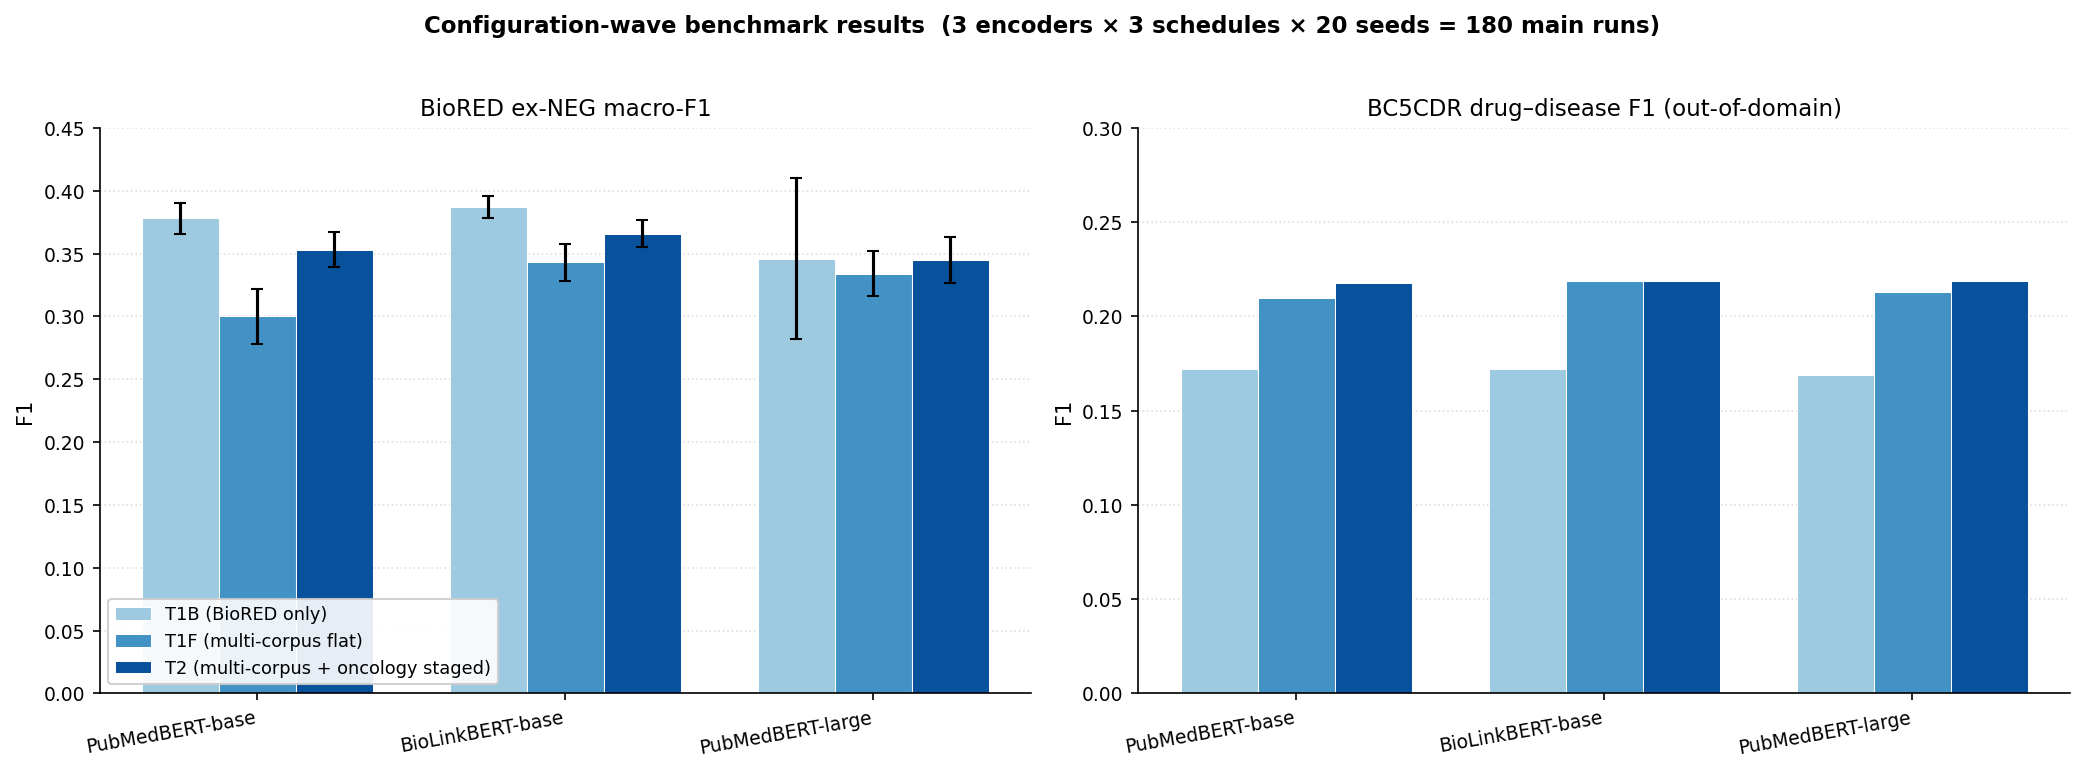
\includegraphics[width=\textwidth]{figures/fig2_training_configs_benchmarks.png}
\caption{Configuration wave: BioRED ex-NEG F1 (left) and BC5CDR
drug--disease F1 (right) by encoder $\times$ schedule. Bars are
20-seed means; error bars are within-cell SDs.}
\label{fig:f2}
\end{figure}

\begin{figure}[!ht]
\centering
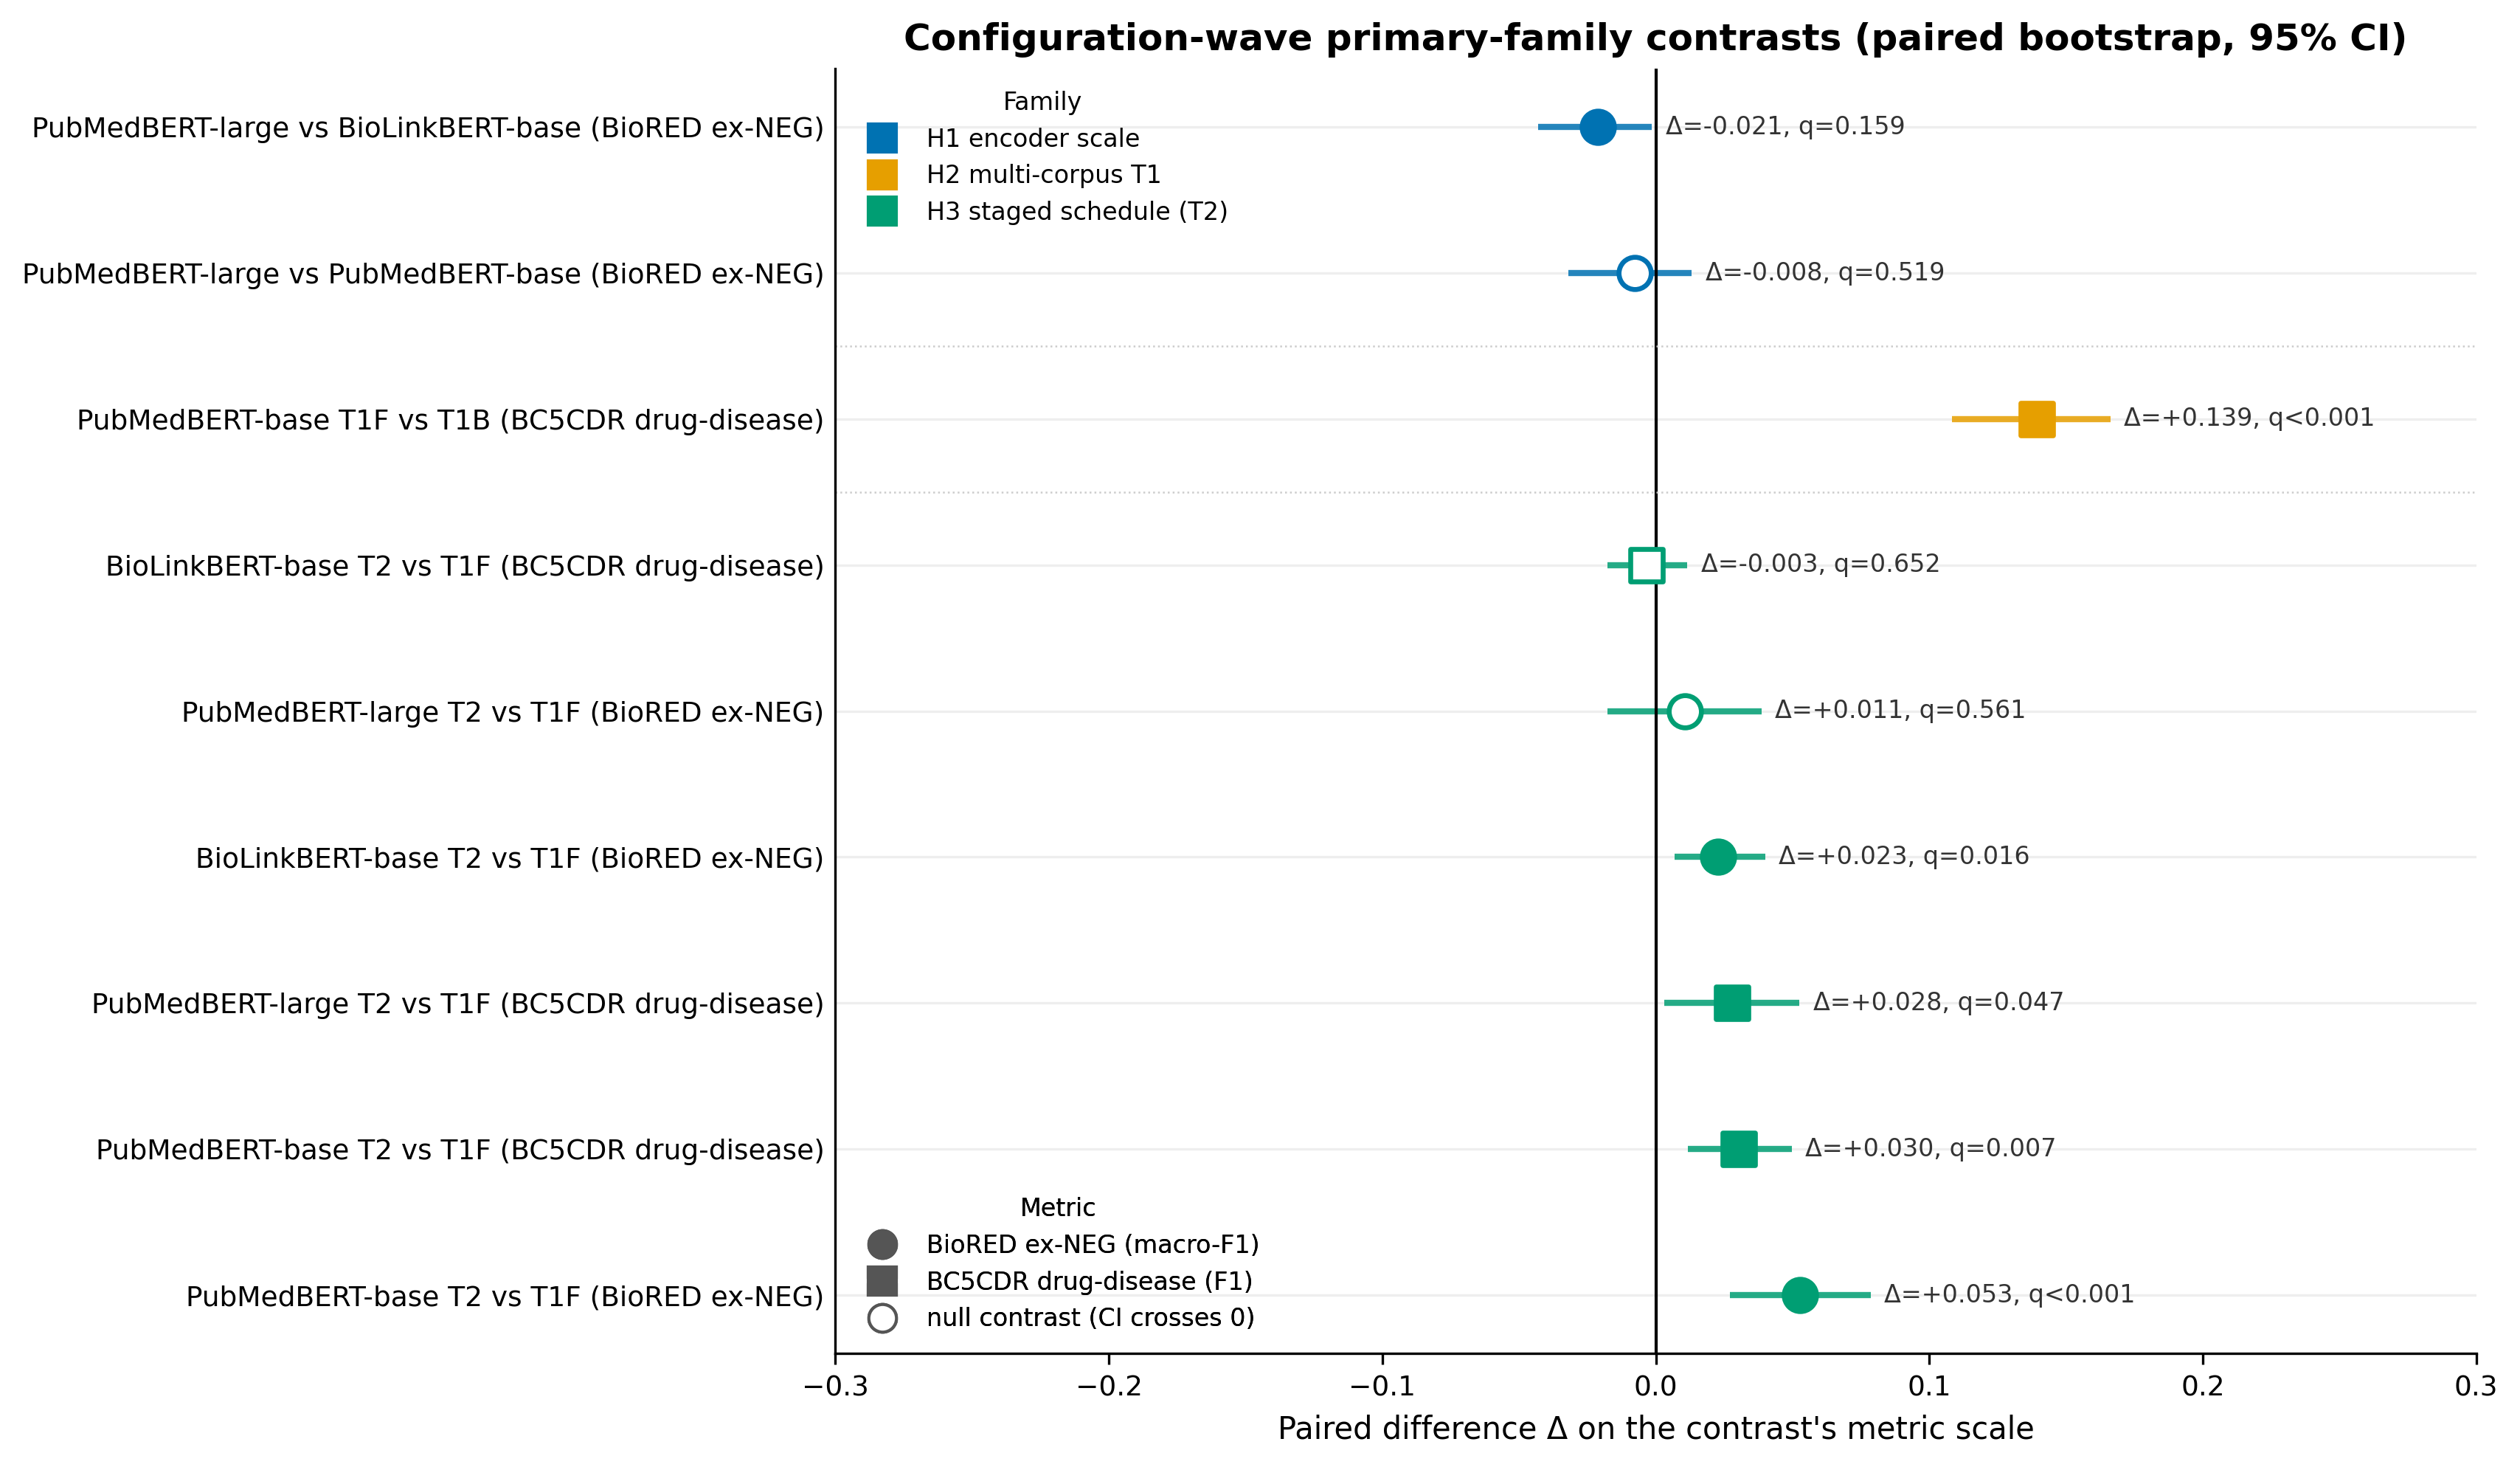
\includegraphics[width=\textwidth]{figures/fig2_forest_plot.png}
\caption{Forest plot of the nine primary-family configuration-wave
contrasts. Markers: circle = BioRED ex-NEG macro-F1; square =
BC5CDR drug--disease F1. Filled = CI excludes zero; open = null.}
\label{fig:f3}
\end{figure}

% =====================================================
\subsection{Audit-metric robustness (RQ3)}
\label{sec:results-rq3}

The encoder \(\times\) audit-metric interaction explained 0.3\% of
variance. Audit-metric choice changed absolute scale but did not
invert the encoder ordering (BioLinkBERT-base \(\approx\)
PubMedBERT-large \(>\) PubMedBERT-base across all three metrics);
the per-encoder profile across the three audit metrics is in
Figure~\ref{fig:s4-kb-profiles} (Supplement~\ref{supp:figures}).

% =====================================================
\subsection{Benchmark--KB coupling (RQ4)}
\label{sec:results-rq4}

\paragraph{Variance asymmetry.}
In the schema-comparison wave, design levers (schema, encoder, and
their interaction) explained 91.9\% of BioRED ex-NEG F1 variance
but only 40.3\% of KB argmax accuracy variance (\(R_A\approx2.28\)).
In the configuration wave the direction of the imbalance reversed:
encoder, schedule, and their interaction explained 14.2\% of
benchmark variance but 66.5\% of KB variance (\(R_B=0.21\);
cluster-bootstrap 95\% CI [0.028, 0.990]). The upper CI bound sits
immediately below unity, so we describe this as a point-estimate
direction reversal consistent with heterogeneous coupling rather
than a confirmed reversal: the test is at the boundary at the
realised cell count. The configuration-wave asymmetry is
concentrated in the schedule term, which explained 59.6\% of KB
variance but only 8.2\% of benchmark variance --- a roughly
seven-fold gap (Figure~\ref{fig:f4}; Supplement~F).

\paragraph{Rank inversion among benchmark-tied pairs.}
Of the 36 unordered configuration-cell pairs, 18 satisfied the
pre-registered matching radius \(\rho=0.03\) on BioRED ex-NEG
(approximately one schema-wave within-cell BioRED SD). Among those
18 benchmark-tied pairs, the median absolute KB argmax accuracy
difference was 0.16 and the rank-inversion rate was 0.50
(cluster-bootstrap 95\% CI [0.14, 0.83]; Clopper--Pearson exact
binomial CI [0.26, 0.74]; Figure~\ref{fig:f4}). A sensitivity
sweep over \(\rho \in \{0.01, 0.03, 0.05\}\) held the rate within
0.50--0.55 (Supplement~H). The interval does not exclude
chance-level KB ordering among benchmark-tied cells; under the
present design we read that as the substantive finding rather than
as a precision-limited null.

\paragraph{Mechanism-stratified slopes.}
All five pre-registered coupling slopes had bootstrap CI widths above
the 0.30 reportability gate and are reported as not estimable. The
configuration-arm slope was \(\beta=-3.0\) (95\% CI
[\(-13.0, +4.5\)]); the remaining four are in Supplement~G. The
reliability ceiling (\S\ref{sec:stats}) constrains slope estimation
at the realised cell counts; we draw the RQ4 coupling claim from the
variance decomposition and rank-inversion analyses above.

\begin{figure}[!ht]
\centering
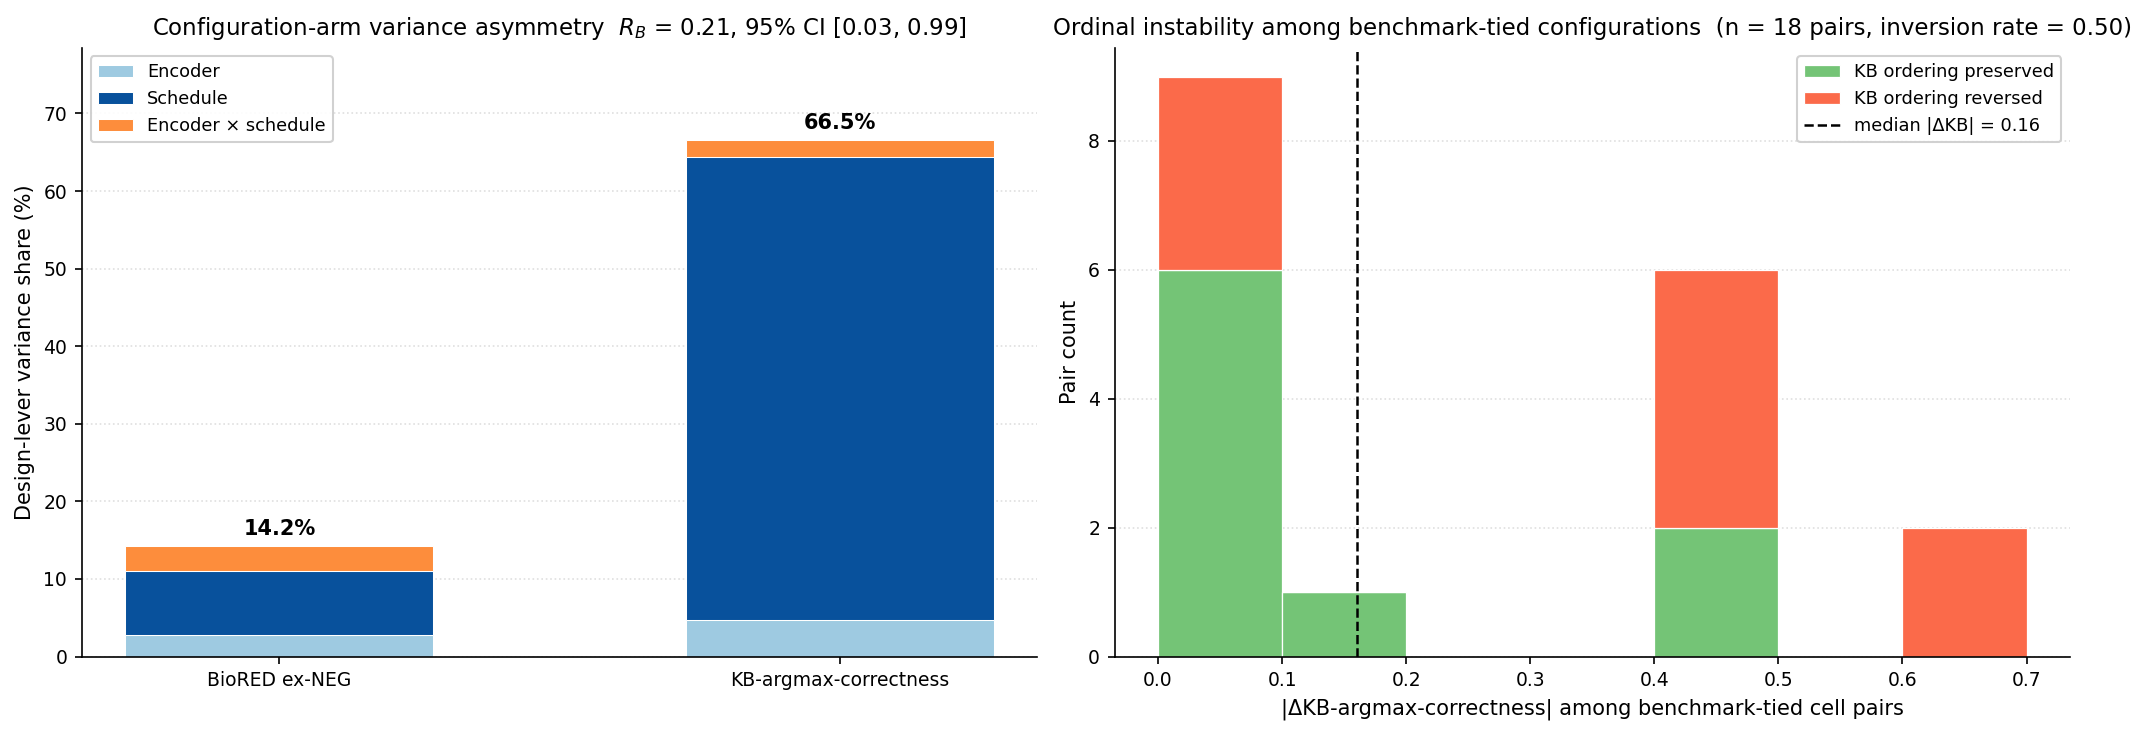
\includegraphics[width=\textwidth]{figures/fig4_variance_asymmetry_and_ordinal.png}
\caption{Left: design-lever variance shares for BioRED ex-NEG F1
and KB argmax accuracy in the configuration wave. Right:
$|\Delta\text{KB}|$ distribution among benchmark-tied cell pairs
($\rho=0.03$).}
\label{fig:f4}
\end{figure}

% =====================================================
\subsection{LoRA falsification}
\label{sec:results-lora}

All three pre-registered LoRA configurations collapsed to
predicting only the negative class (macro-F1 = 0.126, the trivial
baseline); standard fine-tuning learned meaningful predictions
within approximately 512 training steps (macro-F1 \(\approx\) 0.51).
We declared the LoRA comparison a methodological null
(Supplement~I).

\section{Discussion}
\label{sec:discussion}

Benchmark F1 tracked KB yield for some design levers and not
others. Multi-corpus training and oncology-projected staging
improved out-of-domain benchmark generalisation, but those gains
did not translate uniformly to KB surfacing across encoder-schedule
cells. The disagreement concentrated in the training-schedule arm:
schedule explained 59.6\% of KB-argmax-accuracy variance but only
8.2\% of BioRED ex-NEG variance --- a roughly seven-fold gap.

Benchmark scores and KB audits measure overlapping but
non-identical constructs, and divergence under a specific design
lever is informative rather than disqualifying
\citep{lawlor2017triangulation,liugaunt2024asq}. BioRED measures
relation-type discrimination across a broad vocabulary on a topic
mix that is not oncology-specific; the CIViC audit measures
correctness on a narrow oncology subdomain with pre-identified
entity spans. Disagreement between the two scores does not
invalidate either; it shows that they answer different evaluation
questions and respond differently to specific design levers.

One plausible mechanism for the configuration-wave asymmetry is
sample-mix mismatch: CIViC targets concentrate in a narrow oncology
subdomain, whereas the BioRED test set spans a broader topic mix. Schedule
changes that add oncology-projected training shift model behaviour
in the subdomain the KB targets occupy densely but the benchmark
samples sparsely. This account is consistent with the seven-fold
schedule gap; we did not test it directly.

The inter-annotator audit (\S\ref{sec:results-iaa}) sharpens this
account. The heuristic projection over-attributes positive labels
to abstracts where one side of the CIViC-cited (drug, gene) pair is
not literally named, so KB argmax accuracy rewards positive
prediction even when the supporting evidence is not in the
abstract. All seven disagreements clustered on EGFR-pathway TKIs
and the HSP90 inhibitor tanespimycin. Oncology-projected training
plausibly increases positive predictions on these abstracts, so
part of the schedule lever's visibility on the KB metric may be
artefactual. This is a directional caveat; we did not test it
directly.

For clinical KB curation pipelines, the practical implication is to
treat benchmark F1 and a lightweight KB-anchor audit as two
parallel selection inputs. Configuration pairs within one
schema-wave BioRED SD of each other disagreed on KB argmax accuracy
by 0.16 points at the median, with half reversing their ranking, so
benchmark-alone selection is unreliable when the candidates differ
in training schedule. Training schedule therefore deserves more
attention than encoder scale for oncology curation pipelines. We
used 162 CIViC targets with pre-identified entity spans, requiring
no new annotation; the audit code and pre-registration are released
so that other curated oncology KBs (e.g., OncoKB, CancerMine) can
be substituted by replacing the source loader.

\paragraph{Limitations.}
The within-cell standard deviation of KB argmax accuracy (0.17)
is large relative to most paired contrasts we report; this widens
confidence intervals at our cell counts and renders the five
pre-registered coupling slopes inconclusive at the pre-registered
CI-width gate (\S\ref{sec:results-rq4}). The inter-annotator
agreement bound (\(\kappa=0.56\)) indicates moderate annotation
noise, and the seven disagreements concentrated on EGFR-pathway
TKIs would mechanically widen variance estimates in the schedule
arm. The second annotator was a large language model rather than an
independent human curator; \(\kappa=0.56\) should therefore be read
as a lower bound on agreement with an expert curator, and a
blinded human spot check on the same 30 targets is planned
follow-up. We evaluated against a single oncology KB;
generalisation to other clinical subdomains is untested. We
restricted to encoder-only models; an exploratory GPT-4o-mini KB baseline is summarised in Supplement~\ref{supp:llm-phase-d}.
There, GPT-4o-mini exceeds the always-DGR trivial baseline by only 0.04 on the 162-set, and reproduces the heuristic projector's label on all 7 IAA-disagreement targets; we read this as label-space artefact rather than evidence of LLM superiority on the underlying relation-discrimination task.
Other
follow-up work covers a wider LoRA sweep, multi-KB replication,
and a curator-adjudicated subset of the 162 CIViC targets to test
the directional-bias mechanism above.

\section{Conclusion}
\label{sec:conclusion}

In this pre-registered factorial study of cancer assertion
extraction, benchmark F1 and KB-surfacing yield agreed on encoder
scale (both null) and on multi-corpus training (both positive) but
diverged on training schedule. Half of benchmark-tied configuration
pairs reversed their KB ranking. Clinical KB curation pipelines
should pair benchmark scoring with a lightweight KB-anchor audit
against 100--200 curator-validated assertions; the audit protocol,
code, and pre-registration are openly released.


% =============================================================
% BACK MATTER
% =============================================================
\section*{Ethical approval}
This study used only publicly available data: the BioRED, DrugProt,
and BC5CDR relation-extraction corpora; MeSH metadata from PubMed;
and curator-validated oncology assertions from the open CIViC
database. No human-subject data were collected or processed.
Institutional review board approval was therefore not required; the
work was conducted under University of Bristol research-integrity
policy.

\section*{Data and code availability}
% =============================================================
% Data and Code Availability
% =============================================================

The pre-registration document, post-lock amendment log, and all
training and analysis code are openly available at
\url{https://github.com/MRCIEU/assertion_extraction}. The repository
release tag for this manuscript is \code{v1.0-jamia-submission}.
Training data, model checkpoints, and per-run result files are not
included in the repository. All training corpora (BioRED
\citep{luo2022biored}, DrugProt \citep{miranda2023drugprot}, BC5CDR
\citep{li2016bc5cdr}) are publicly available under their respective
distribution licences, and the CIViC oncology evidence database
\citep{griffith2017civic} is distributed under CC0 via
\url{https://civicdb.org}. No internal F.\ Hoffmann-La Roche Ltd
data was used; all analyses are reproducible from the released code
and the public corpora alone.

\section*{Funding}
% Funding sources and grant numbers to be confirmed with supervisors.


\section*{Author contributions}
% CRediT author contributions to be confirmed with supervisors.


\section*{Acknowledgements}
% Acknowledgements to be confirmed with supervisors.


% =============================================================
% REFERENCES
% =============================================================
\bibliographystyle{unsrtnat}
\bibliography{references}

\end{document}